% !Rnw weave = Sweave
\documentclass[xcolor={table}, handout]{beamer}

% Allow compilation from repo root or from /slides.
\newcommand{\plscassetpath}{../assets}
\IfFileExists{../assets/pres-template_MOW.sty}{}{%
  \renewcommand{\plscassetpath}{assets}%
}
\newcommand{\plscbibpath}{../assets/PLSC40601}
\IfFileExists{../assets/PLSC40601.bib}{}{%
  \renewcommand{\plscbibpath}{assets/PLSC40601}%
}

\RequirePackage{\plscassetpath/pres-template_MOW}
\graphicspath{{./}{slides/}{assets/}{../assets/}}
\usepackage{colortbl}

%--------------------------------------------------------------------------
% Specific to this document ---------------------------------------
\RequirePackage{mathtools}
\RequirePackage{tabularray}
\NewColumnType{M}[1]{Q[m,c,#1]}
\newcommand{\figpath}[1]{\plscassetpath/#1}

\makeatletter
\def\normaljustify{%
  \let\\\@centercr
  \rightskip\z@skip
  \leftskip\z@skip%
  \parfillskip=0pt plus 1.0fil\relax
}
\makeatother

%--------------------------------------------------------------------------
% \setbeamercovered{transparent}

%%%%%%%%%%%%%%%%%%%%%%%%%%%%%%%%%%%
\setlength{\tabcolsep}{1.3pt}
\title{PLSC 40601}
\subtitle{Week 7: Efficient estimation.}
\date{Spring 2026}
\author{Molly Offer-Westort}
\institute{Department of Political Science, \\University of Chicago}

\usepackage{Sweave}
\begin{document}

%-------------------------------------------------------------------------------%
\frame{\titlepage
\thispagestyle{empty}
}
%-------------------------------------------------------------------------------%
\begin{transitionframe}
\centering

\LARGE \textcolor{white}{Some asymptotic language.}

\end{transitionframe}

%%%%%NOTE%%%%%
\note{
\scriptsize \singlespacing

%\begin{wideitemize}
%\item xxx
%\end{wideitemize}
}
%-------------------------------------------------------------------------------%
\begin{frame}{Convergence}
Review \cite{lehmann1999elements} Chapter 2
\vskip 0.2cm

\begin{wideitemize}
\item A deterministic sequence $a_n$ converges to $a$, written
\[
a_n\rightarrow a,
\]
if:
\[
\forall \varepsilon>0,\ \exists N\in\mathbb{N}
\text{ such that for all } n\geq N,\ |a_n-a|<\varepsilon.
\]\pause
\item I.e., for every tolerance $\varepsilon$, no matter how small, there is some point $N$ after which every term of the sequence is within $\varepsilon$ of the limit $a$.
\end{wideitemize}

\end{frame}

%%%%%NOTE%%%%%
\note{
\scriptsize \singlespacing

%\begin{wideitemize}
%\item xxx
%\end{wideitemize}
}
%-------------------------------------------------------------------------------%
\begin{frame}{Convergence in probability}

\begin{wideitemize}
\item A sequence of random variables $X_n$ converges in probability to $X$ if, for every $\varepsilon>0$,
\[
\Pr[|X_n-X|>\varepsilon]\rightarrow 0.
\]\pause
\item We write
\[
X_n \overset{p}{\rightarrow} X.
\]\pause
\item For an estimator:
\[
\hat\theta_n \overset{p}{\rightarrow} \theta_0
\]
means $\hat\theta_n$ is consistent for $\theta_0$.
\end{wideitemize}

\end{frame}

%%%%%NOTE%%%%%
\note{
\scriptsize \singlespacing

%\begin{wideitemize}
%\item xxx
%\end{wideitemize}
}
%-------------------------------------------------------------------------------%
\begin{frame}{Convergence in distribution}

\begin{wideitemize}
\item A sequence $X_n$ converges in distribution to $X$ if
\[
F_n(x)\rightarrow F(x)
\]
at every continuity point $x$ of the limiting distribution function $F$.\pause
\item We write
\[
X_n \overset{d}{\rightarrow} X.
\]OR 
\[
X_n \rightsquigarrow X.
\]
\pause
\item E.g., for asymptotic normality:
\[
\sqrt{n}(\hat\theta_n-\theta_0)
  \overset{d}{\rightarrow}
  N(0,V).
\]\pause
\item Intuition: the shape of the sampling distribution stabilizes.
\end{wideitemize}

\end{frame}

%%%%%NOTE%%%%%
\note{
\scriptsize \singlespacing

%\begin{wideitemize}
%\item xxx
%\end{wideitemize}
}
%-------------------------------------------------------------------------------%
\begin{frame}{Big-oh and little-oh}

\begin{wideitemize}
\item For deterministic sequences, $a_n=O(b_n)$ means
\[
\left|\frac{a_n}{b_n}\right|
\]
is eventually bounded.\pause
\item $a_n=o(b_n)$ means
\[
\frac{a_n}{b_n}\rightarrow 0.
\]\pause
\item So:
\[
a_n=O(n^{-1/2})
\]
means $a_n$ is no larger than root-$n$ order.\pause
\item And:
\[
a_n=o(n^{-1/2})
\]
means $a_n$ is negligible relative to root-$n$ order.
\end{wideitemize}

\end{frame}

%%%%%NOTE%%%%%
\note{
\scriptsize \singlespacing

%\begin{wideitemize}
%\item xxx
%\end{wideitemize}
}
%-------------------------------------------------------------------------------%
\begin{frame}{Stochastic order notation}

\begin{wideitemize}
\item For random sequences, $X_n=O_p(a_n)$ means
\[
\frac{X_n}{a_n}
\]
is bounded in probability.\pause
\item $X_n=o_p(a_n)$ means
\[
\frac{X_n}{a_n}\overset{p}{\rightarrow}0.
\]\pause
\item Examples:
\[
\hat\theta_n-\theta_0=O_p(n^{-1/2})
\]
means root-$n$ consistency.\pause
\item
\[
\hat\theta_n-\theta_0=o_p(1)
\]
means ordinary consistency.
\end{wideitemize}

\end{frame}

%%%%%NOTE%%%%%
\note{
\scriptsize \singlespacing

%\begin{wideitemize}
%\item xxx
%\end{wideitemize}
}
%-------------------------------------------------------------------------------%
\begin{frame}{Why rates matter here}

\begin{wideitemize}
\item Efficient-estimation arguments separate a leading term from a remainder:
\[
\hat\psi-\psi_0
  =
  \text{first-order term}
  +
  \text{remainder}.
\]\pause
\item We want the remainder to be negligible:
\[
\text{remainder}=o_p(n^{-1/2}).
\]\pause
\item In doubly robust estimators, the remainder often behaves like a product of nuisance errors:
\[
\|\hat m-m_0\|\|\hat e-e_0\|.
\]\pause
\item That product can be small enough even when each nuisance estimate is slower than root-$n$.
\end{wideitemize}

\end{frame}

%%%%%NOTE%%%%%
\note{
\scriptsize \singlespacing

%\begin{wideitemize}
%\item xxx
%\end{wideitemize}
}
%-------------------------------------------------------------------------------%
\begin{frame}{The empirical measure}

\begin{wideitemize}
\item The empirical measure puts mass $1/n$ on each observed data point:
\[
\mathbb{P}_n
  =
  \frac{1}{n}\sum_{t=1}^n \delta_{O_t}.
\]\pause
\item For a set $A$:
\[
\mathbb{P}_n[A]
  =
  \frac{1}{n}\sum_{t=1}^n \mathbbm{1}(O_t\in A).
\]\pause
\item For a function $f$:
\[
\mathbb{P}_n f
  =
  \frac{1}{n}\sum_{t=1}^n f(O_t),
\qquad
P_0 f
  =
  \mathbb{E}_{P_0}[f(O)].
\]\pause
\item This lets us write sample averages as integrals with respect to $\mathbb{P}_n$.
\end{wideitemize}

\end{frame}

%%%%%NOTE%%%%%
\note{
\scriptsize \singlespacing

%\begin{wideitemize}
%\item xxx
%\end{wideitemize}
}
%-------------------------------------------------------------------------------%
\begin{frame}{Empirical-process notation}

\begin{wideitemize}
\item The gap between sample and population averages is
\[
(\mathbb{P}_n-P_0)f
  =
  \frac{1}{n}\sum_{t=1}^n f(O_t)
  -
  \mathbb{E}_{P_0}[f(O)].
\]\pause
\item The central limit theorem gives, for fixed $f$,
\[
\sqrt{n}(\mathbb{P}_n-P_0)f
  \overset{d}{\rightarrow}
  N\{0,\Var_{P_0}[f(O)]\}.
\]\pause
\item Influence-function estimators are built so their leading term has this form.
\end{wideitemize}

\end{frame}

%%%%%NOTE%%%%%
\note{
\scriptsize \singlespacing

%\begin{wideitemize}
%\item xxx
%\end{wideitemize}
}
%-------------------------------------------------------------------------------%
\begin{transitionframe}
\centering

\LARGE \textcolor{white}{Model classes.}

\end{transitionframe}

%%%%%NOTE%%%%%
\note{
\scriptsize \singlespacing

%\begin{wideitemize}
%\item xxx
%\end{wideitemize}
}
%-------------------------------------------------------------------------------%
\begin{frame}{What is a statistical model?}

\begin{wideitemize}
\item We observe
\[
Z_1,\dots,Z_n \overset{iid}{\sim} P_0,
\]
where $P_0$ is the unknown true data-generating distribution.\pause
\item A \textbf{statistical model} is a set of distributions:
\[
\mathcal{P}=\{P: P \text{ is allowed by our assumptions}\}.
\]\pause
\item Saying
\[
P_0\in\mathcal{P}
\]
means the true distribution is one of the distributions allowed by the model.
\end{wideitemize}

\end{frame}

%%%%%NOTE%%%%%
\note{
\scriptsize \singlespacing

%\begin{wideitemize}
%\item xxx
%\end{wideitemize}
}
%-------------------------------------------------------------------------------%
\begin{frame}{A model is a set of possible worlds}

\begin{wideitemize}
\item Here, a is a mathematical set of possible worlds.\pause
\item The stronger the assumptions, the smaller the set $\mathcal{P}$.\pause
\item The weaker the assumptions, the larger the set $\mathcal{P}$.
\end{wideitemize}

\end{frame}

%%%%%NOTE%%%%%
\note{
\scriptsize \singlespacing

%\begin{wideitemize}
%\item xxx
%\end{wideitemize}
}
%-------------------------------------------------------------------------------%
\begin{frame}{Three kinds of models}

\begin{wideitemize}
\item \textbf{Parametric}: $\mathcal{P}$ is indexed by finitely many parameters.\pause
\item \textbf{Nonparametric}: $\mathcal{P}$ is infinite-dimensional, often very large.\pause
\item \textbf{Semiparametric}: the target is finite-dimensional, but the nuisance structure is infinite-dimensional.
\end{wideitemize}

\end{frame}

%%%%%NOTE%%%%%
\note{
\scriptsize \singlespacing

%\begin{wideitemize}
%\item xxx
%\end{wideitemize}
}
%-------------------------------------------------------------------------------%
\begin{frame}{Parametric models}

\begin{wideitemize}
\item A \textbf{parametric model} is indexed by a finite-dimensional parameter:
\[
\mathcal{P}
  =
  \{P_\theta:\theta\in\Theta\subseteq\mathbb{R}^d\}.
\]\pause
\item Once $\theta$ is known, the whole distribution is known.\pause
\item Normal example:
\[
\mathcal{P}
  =
  \{N(\mu,\sigma^2):\mu\in\mathbb{R},\sigma^2>0\}.
\]\pause
\item Saying $P_0\in\mathcal{P}$ means the true distribution is normal for some $\mu$ and $\sigma^2$.\pause
\item Parametric models are restrictive, but they give sharp benchmarks like Fisher information.
\end{wideitemize}

\end{frame}

%%%%%NOTE%%%%%
\note{
\scriptsize \singlespacing

%\begin{wideitemize}
%\item xxx
%\end{wideitemize}
}
%-------------------------------------------------------------------------------%
\begin{frame}{Semiparametric models}

\begin{wideitemize}
\item A \textbf{semiparametric model} has a finite-dimensional target and infinite-dimensional nuisance components.\pause
\item Example target:
\[
\psi_0=\mathbb{E}[Y(1)-Y(0)].
\]\pause
\item Under identification, $\psi_0=\Psi(P_0)$, but $P_0$ contains nuisance functions such as
\[
\mu_a(x)=\mathbb{E}[Y\mid A=a,X=x],
\qquad
e(x)=\Pr[A=1\mid X=x].
\]\pause
\item We care about $\psi_0$, but we may estimate $\mu_a$ and $e$ flexibly with ML.
\end{wideitemize}

\end{frame}

%%%%%NOTE%%%%%
\note{
\scriptsize \singlespacing

%\begin{wideitemize}
%\item xxx
%\end{wideitemize}
}
%-------------------------------------------------------------------------------%
\begin{frame}{Regression restrictions: semiparametric}

\begin{wideitemize}
\item Some models restrict part of the distribution rather than every feature of it.\pause
\item Example:
\[
\mathbb{E}_{P_0}[Y\mid X]=\beta_0+\beta_1X.
\]\pause
\item Then $\mathcal{P}$ is the set of distributions whose conditional mean of $Y$ given $X$ is linear.\pause
\item Saying $P_0\in\mathcal{P}$ means the true conditional mean is linear.\pause
\item This is usually \textbf{semiparametric}: $\beta$ is finite-dimensional, but the distribution of $X$, the error distribution, and higher moments remain unrestricted.
\end{wideitemize}

\end{frame}

%%%%%NOTE%%%%%
\note{
\scriptsize \singlespacing

%\begin{wideitemize}
%\item xxx
%\end{wideitemize}
}
%-------------------------------------------------------------------------------%
\begin{frame}{When regression becomes parametric}

\begin{wideitemize}
\item To make the regression model fully parametric, we would need stronger assumptions, e.g.
\[
Y\mid X \sim N(\beta_0+\beta_1X,\sigma^2).
\]\pause
\item Then a finite-dimensional parameter determines the full conditional distribution:
\[
\theta=(\beta_0,\beta_1,\sigma^2).
\]
\end{wideitemize}

\end{frame}

%%%%%NOTE%%%%%
\note{
\scriptsize \singlespacing

%\begin{wideitemize}
%\item xxx
%\end{wideitemize}
}
%-------------------------------------------------------------------------------%
\begin{frame}{Nonparametric models}

\begin{wideitemize}
\item A \textbf{nonparametric model} allows the distribution to vary over a much larger, infinite-dimensional class.\pause
\item In the simplest case:
\[
\mathcal{P}
  =
  \{P: P \text{ is any probability distribution on the sample space}\}.
\]\pause
\item Then $P_0\in\mathcal{P}$ is very weak: it only says the truth is a valid probability distribution.
\end{wideitemize}

\end{frame}

%%%%%NOTE%%%%%
\note{
\scriptsize \singlespacing

%\begin{wideitemize}
%\item xxx
%\end{wideitemize}
}
%-------------------------------------------------------------------------------%
\begin{frame}{Nonparametric restrictions}

\begin{wideitemize}
\item Example:
\[
\mathcal{P}
  =
  \{P: \mathbb{E}_P[Y^2]<\infty\}.
\]\pause
\item The model does not say $Y$ is normal, linear in $X$, logistic, or indexed by a finite number of coefficients.\pause
\item This flexibility is useful, but it usually makes estimation and inference harder.
\item Later restrictions may add smoothness or sparsity assumptions.
\end{wideitemize}

\end{frame}

%%%%%NOTE%%%%%
\note{
\scriptsize \singlespacing

%\begin{wideitemize}
%\item xxx
%\end{wideitemize}
}
%-------------------------------------------------------------------------------%

\begin{frame}{Functionals}

\begin{wideitemize}
\item A \textbf{functional} is a function whose input is itself a whole distribution, curve, density, regression function, or other infinite-dimensional object.\pause
\item Ordinary function:
\[
f:x\mapsto f(x).
\]\pause
\item Functional:
\[
\Psi:P\mapsto \Psi(P).
\]\pause
\item In semiparametric causal inference, the target is usually a functional of the observed-data distribution:
\[
\psi_0=\Psi(P_0).
\]
\end{wideitemize}

\end{frame}

%%%%%NOTE%%%%%
\note{
\scriptsize \singlespacing

%\begin{wideitemize}
%\item xxx
%\end{wideitemize}
}
%-------------------------------------------------------------------------------%
\begin{frame}{Function versus functional}

\begin{wideitemize}
\item $\mu(x)$ is a function:
\[
x \mapsto \mu(x).
\]\pause
\item It takes a covariate value $x$ as input and returns a number.\pause
\item $\mathbb{E}[\mu(X)]$ is a functional of $P$:
\[
\Psi(P)
  =
  \int \mu_P(x)\,dP_X(x).
\]\pause
\item It depends on the whole regression function $\mu_P(\cdot)$ and on the distribution of $X$.
\end{wideitemize}

\end{frame}

%%%%%NOTE%%%%%
\note{
\scriptsize \singlespacing

%\begin{wideitemize}
%\item xxx
%\end{wideitemize}
}
%-------------------------------------------------------------------------------%
\begin{frame}{Why semiparametric language matters}

\begin{wideitemize}
\item Causal ML usually does not ask us to estimate the whole distribution $P_0$ well.\pause
\item It asks us to estimate a lower-dimensional target $\Psi(P_0)$ well.\pause
\item The nuisance functions can be high-dimensional or nonparametric.\pause
\item Efficient estimation is about extracting first-order information for the target while reducing sensitivity to nuisance-estimation error.
\end{wideitemize}

\end{frame}

%%%%%NOTE%%%%%
\note{
\scriptsize \singlespacing

%\begin{wideitemize}
%\item xxx
%\end{wideitemize}
}
%-------------------------------------------------------------------------------%
\begin{transitionframe}
\centering

\LARGE \textcolor{white}{Fisher information.}

\end{transitionframe}

%%%%%NOTE%%%%%
\note{
\scriptsize \singlespacing

%\begin{wideitemize}
%\item xxx
%\end{wideitemize}
}
%-------------------------------------------------------------------------------%
\begin{frame}{Why start with Fisher information?}

\begin{wideitemize}
\item We want to estimate a target parameter $\theta$ from data $O_1,\dots,O_n$.\pause
\item Many estimators are consistent: they converge to the right answer.\pause
\item Efficiency asks a sharper question:
among regular estimators,
how small can the asymptotic variance be?
\pause
\item Fisher information gives the cleanest version of this question in parametric models. \hfill \cite{lehmann1999elements} Section 7.2
\end{wideitemize}

\end{frame}

%%%%%NOTE%%%%%
\note{
\scriptsize \singlespacing

%\begin{wideitemize}
%\item xxx
%\end{wideitemize}
}
%-------------------------------------------------------------------------------%
\begin{frame}{Parametric model}

\begin{wideitemize}
\item Suppose observations are i.i.d.:
\[
O_1,\dots,O_n \sim P_{\theta_0}, \qquad \theta_0 \in \Theta \subset \mathbb{R}.
\]\pause
\item The model says the whole distribution is indexed by one unknown number:
\[
\mathcal{P} = \{P_\theta: \theta \in \Theta\}.
\]\pause
\item If $p_\theta(o)$ is the density or mass function, the likelihood is
\[
L_n(\theta)=\prod_{t=1}^n p_\theta(O_t),
\]
and the log-likelihood is
\[
\ell_n(\theta)=\sum_{t=1}^n \log p_\theta(O_t).
\]
\end{wideitemize}

\end{frame}

%%%%%NOTE%%%%%
\note{
\scriptsize \singlespacing

%\begin{wideitemize}
%\item xxx
%\end{wideitemize}
}
%-------------------------------------------------------------------------------%
\begin{frame}{The score}

\begin{wideitemize}
\item The score is the derivative of the log likelihood contribution:
\[
s_\theta(O_t)
  =
  \frac{\partial}{\partial \theta}\log p_\theta(O_t).
\]\pause
\item The sample score is
\[
S_n(\theta)
  =
  \frac{\partial}{\partial \theta}\ell_n(\theta)
  =
  \sum_{t=1}^n s_\theta(O_t).
\]\pause
\item The score tells us the local direction in which the data push the parameter estimate.
\end{wideitemize}

\end{frame}

%%%%%NOTE%%%%%
\note{
\scriptsize \singlespacing

%\begin{wideitemize}
%\item xxx
%\end{wideitemize}
}
%-------------------------------------------------------------------------------%
\begin{frame}{A key property}

\begin{wideitemize}
\item Under regularity conditions, the score has mean zero at the true parameter:
\[
\mathbb{E}_{\theta_0}[s_{\theta_0}(O)]=0.
\]\pause
\item Intuition:
\[
\int p_\theta(o)d o = 1
\quad \Rightarrow \quad
\frac{\partial}{\partial \theta}\int p_\theta(o)d o = 0.
\]\pause
\item Since by the chain rule
\[
\frac{\partial}{\partial \theta}p_\theta(o)
  =
  p_\theta(o)\frac{\partial}{\partial \theta}\log p_\theta(o),
\]
the average score must be zero.
\end{wideitemize}

\end{frame}

%%%%%NOTE%%%%%
\note{
\scriptsize \singlespacing

%\begin{wideitemize}
%\item xxx
%\end{wideitemize}
}
%-------------------------------------------------------------------------------%
\begin{frame}{Fisher information}

\begin{wideitemize}
\item Fisher information is the variance of the score.\pause
\item Since the score is mean zero, this variance can be written as
\[
I(\theta)
  =
  \mathbb{E}_{\theta}[s_\theta(O)^2].
\]\pause
\item Equivalently, under regularity conditions,
\[
I(\theta)
  =
  -\mathbb{E}_{\theta}
  \left[
  \frac{\partial^2}{\partial \theta^2}\log p_\theta(O)
  \right].
\]\pause
\item For $n$ i.i.d. observations:
\[
I_n(\theta)=n I(\theta).
\]\pause
\item More information means the likelihood is more sharply curved around the truth.
\end{wideitemize}

\end{frame}

%%%%%NOTE%%%%%
\note{
\scriptsize \singlespacing

%\begin{wideitemize}
%\item xxx
%\end{wideitemize}
}
%-------------------------------------------------------------------------------%
\begin{frame}{Likelihood curvature}

\centering
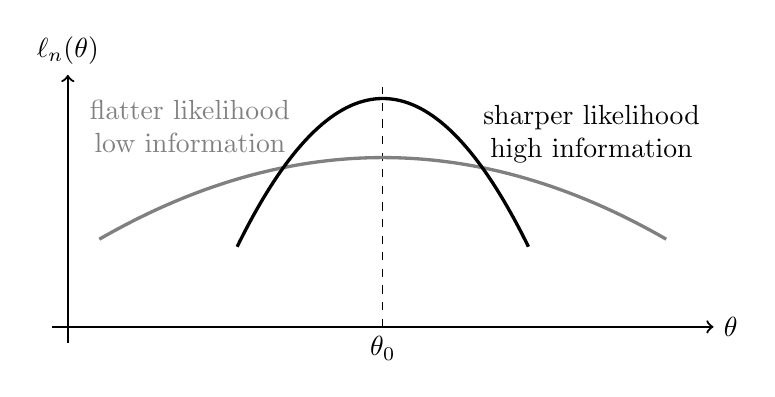
\begin{tikzpicture}[x=1cm,y=1cm]
  \draw[->, thick] (-4.2,0) -- (4.2,0) node[right] {$\theta$};
  \draw[->, thick] (-4,-0.2) -- (-4,3.2) node[above] {$\ell_n(\theta)$};

  \draw[dashed] (0,0) -- (0,3.05);
  \node[below] at (0,0) {$\theta_0$};

  \draw[very thick, gray]
    plot[domain=-3.6:3.6,samples=100] (\x,{2.15 - 0.08*\x*\x});
  \node[gray, align=center] at (-2.45,2.55) {flatter likelihood\\low information};

  \draw[very thick, black]
    plot[domain=-1.85:1.85,samples=100] (\x,{2.9 - 0.55*\x*\x});
  \node[black, align=center] at (2.65,2.45) {sharper likelihood\\high information};
\end{tikzpicture}

\vspace{0.2cm}

\begin{wideitemize}
\item Nearby values of $\theta$ are harder to distinguish when the likelihood is flat.\pause
\item Nearby values of $\theta$ are easier to distinguish when the likelihood is sharply curved.
\end{wideitemize}

\end{frame}

%%%%%NOTE%%%%%
\note{
\scriptsize \singlespacing

%\begin{wideitemize}
%\item xxx
%\end{wideitemize}
}
%-------------------------------------------------------------------------------%
\begin{frame}{Example: Bernoulli data}

\begin{wideitemize}
\item Let $O_t \in \{0,1\}$ and
\[
P_\theta[O_t=1]=\theta.
\]\pause
\item Then the probability mass function is
\[
p_\theta(O_t)
  =
  \theta^{O_t}(1-\theta)^{1-O_t}.
\]\pause
\item I.e.,:
\[
O_t=1 \Rightarrow p_\theta(O_t)=\theta,
\qquad
O_t=0 \Rightarrow p_\theta(O_t)=1-\theta.
\]
\end{wideitemize}

\end{frame}

%%%%%NOTE%%%%%
\note{
\scriptsize \singlespacing

%\begin{wideitemize}
%\item xxx
%\end{wideitemize}
}
%-------------------------------------------------------------------------------%
\begin{frame}{Example: Bernoulli score}

\begin{wideitemize}
\item Recall the score is the derivative of the log likelihood contribution:
\[
s_\theta(O_t)
  =
  \frac{\partial}{\partial\theta}\log p_\theta(O_t).
\]\pause
\item For Bernoulli data, the log likelihood contribution is
\[
\log p_\theta(O_t)
  =
  O_t \log(\theta)
  +(1-O_t)\log(1-\theta).
\]\pause
\item Differentiate with respect to $\theta$:
\[
s_\theta(O_t)
  =
  \frac{O_t}{\theta}
  -
  \frac{1-O_t}{1-\theta}.
\]\pause
\item Put over a common denominator:
\[
s_\theta(O_t)
  =
  \frac{O_t-\theta}{\theta(1-\theta)}.
\]
\end{wideitemize}

\end{frame}

%%%%%NOTE%%%%%
\note{
\scriptsize \singlespacing

%\begin{wideitemize}
%\item xxx
%\end{wideitemize}
}
%-------------------------------------------------------------------------------%
\begin{frame}{Bernoulli information: plug in the score}

\small

\begin{wideitemize}
\item Recall Fisher information is the variance of the score:
\[
I(\theta)
  =
  \mathbb{E}_\theta[s_\theta(O_t)^2].
\]\pause
\item We just found:
\[
s_\theta(O_t)
  =
  \frac{O_t-\theta}{\theta(1-\theta)}.
\]\pause
\item Plug that score into the definition:
\[
I(\theta)
  =
  \mathbb{E}_\theta
  \left[
    \left\{
      \frac{O_t-\theta}{\theta(1-\theta)}
    \right\}^2
  \right].
\]\pause
\item The denominator is not random, so it can move outside the expectation:
\[
I(\theta)
  =
  \frac{\mathbb{E}_\theta[(O_t-\theta)^2]}
       {\{\theta(1-\theta)\}^2}.
\]
\end{wideitemize}

\end{frame}

%%%%%NOTE%%%%%
\note{
\scriptsize \singlespacing

%\begin{wideitemize}
%\item xxx
%\end{wideitemize}
}
%-------------------------------------------------------------------------------%
\begin{frame}{Bernoulli information: simplify}

\begin{wideitemize}
\item Since $O_t\sim\text{Bernoulli}(\theta)$,
\[
\mathbb{E}_\theta[O_t]=\theta,
\qquad
\Var_\theta[O_t]=\theta(1-\theta).
\]\pause
\item The numerator is the variance:
\[
\mathbb{E}_\theta[(O_t-\theta)^2]
  =
  \Var_\theta[O_t].
\]\pause
\item Therefore:
\[
I(\theta)
  =
  \frac{\Var_\theta[O_t]}
       {\{\theta(1-\theta)\}^2}
  =
  \frac{1}{\theta(1-\theta)}.
\]\pause
\item So the Fisher information for one observation is
\[
I(\theta)=\frac{1}{\theta(1-\theta)}.
\]
\end{wideitemize}

\end{frame}

%%%%%NOTE%%%%%
\note{
\scriptsize \singlespacing

%\begin{wideitemize}
%\item xxx
%\end{wideitemize}
}
%-------------------------------------------------------------------------------%
\begin{frame}{Information and variance}

\begin{wideitemize}
\item The MLE is $\hat\theta=\bar O$.\pause
\item By the central limit theorem, when $0<\theta_0<1$:
\[
\sqrt{n}(\hat\theta-\theta_0)
  \overset{d}{\rightarrow}
  N\{0,\theta_0(1-\theta_0)\}.
\]\pause
\item Since
\[
I(\theta_0)^{-1}
  =
  \theta_0(1-\theta_0),
\]
the MLE reaches the Fisher-information variance benchmark.\pause
\item This is the basic meaning of parametric efficiency.
\end{wideitemize}

\end{frame}

%%%%%NOTE%%%%%
\note{
\scriptsize \singlespacing

%\begin{wideitemize}
%\item xxx
%\end{wideitemize}
}
%-------------------------------------------------------------------------------%
\begin{frame}{Cram\'er--Rao intuition}

\begin{wideitemize}
\item In a regular parametric model, no regular unbiased estimator can have variance below
\[
\frac{1}{n I(\theta_0)}.
\]\pause
\item More generally, regular asymptotically linear estimators face an asymptotic variance bound.\pause
\item So an efficient estimator is not just consistent.\pause
\item It is as stable as the model allows, to first order:
\[
\sqrt{n}(\hat\theta-\theta_0)
  \overset{d}{\rightarrow}
  N\{0, I(\theta_0)^{-1}\}.
\]
\end{wideitemize}

\end{frame}

%%%%%NOTE%%%%%
\note{
\scriptsize \singlespacing

%\begin{wideitemize}
%\item xxx
%\end{wideitemize}
}
%-------------------------------------------------------------------------------%
\begin{frame}{Kennedy's Theorem 1: setup}

\small

\begin{wideitemize}
\item Cram\'er--Rao gives the familiar variance story; Kennedy states a stronger asymptotic minimax version.\pause
\item Kennedy starts from a smooth parametric model:
\[
\mathcal{P}=\{P_\theta:\theta\in\Theta\}.
\]\pause
\item The target is a smooth function of $\theta$:
\[
\psi(\theta).
\]\pause
\item The theorem asks: how small can the local worst-case MSE be for estimating $\psi(\theta)$?
\end{wideitemize}

\end{frame}

%%%%%NOTE%%%%%
\note{
\scriptsize \singlespacing

%\begin{wideitemize}
%\item xxx
%\end{wideitemize}
}
%-------------------------------------------------------------------------------%
\begin{frame}{Kennedy's Theorem 1: assumptions}

\small

\begin{wideitemize}
\item The score and Fisher information are
\[
s_\theta(Z)
  =
  \frac{\partial}{\partial\theta}\log p_\theta(Z),
\qquad
I_\theta=\Var_\theta[s_\theta(Z)].
\]\pause
\item Assume $P_\theta$ is differentiable in quadratic mean at $\theta$.\pause
\item Assume $I_\theta$ is nonsingular and $\psi(\theta)$ is differentiable.
\end{wideitemize}

\end{frame}

%%%%%NOTE%%%%%
\note{
\scriptsize \singlespacing

%\begin{wideitemize}
%\item xxx
%\end{wideitemize}
}
%-------------------------------------------------------------------------------%
\begin{frame}{Kennedy's Theorem 1: statement}

\small

\begin{wideitemize}
\item For any estimator $\hat\psi$, \citet{kennedy2022semiparametric} states:
\[
\inf_{\delta>0}
\liminf_{n\rightarrow\infty}
\sup_{\|\theta'-\theta\|<\delta}
n\,
\mathbb{E}_{\theta'}
\left[
  \{\hat\psi-\psi(\theta')\}^2
\right]
\geq
\psi'(\theta) I_\theta^{-1} \psi'(\theta)^T.
\]\pause
\item The right-hand side is the parametric efficiency benchmark:
\[
\psi'(\theta) I_\theta^{-1} \psi'(\theta)^T.
\]\pause
\item If $\psi(\theta)=\theta$, this reduces to
\[
I_\theta^{-1}.
\]\pause
\item So the theorem gives the asymptotic local worst-case MSE bound for smooth functions of $\theta$.
\end{wideitemize}

\end{frame}

%%%%%NOTE%%%%%
\note{
\scriptsize \singlespacing

%\begin{wideitemize}
%\item xxx
%\end{wideitemize}
}
%-------------------------------------------------------------------------------%
\begin{frame}{Stronger than Cram\'er--Rao}

\begin{wideitemize}
\item The classical Cram\'er--Rao bound is often stated for unbiased estimators.\pause
\item Kennedy's Theorem 1 is a local asymptotic minimax statement.\pause
\item It allows biased estimators, adaptive estimators, unusual estimators, and arbitrary estimator sequences.\pause
\item The conclusion is stronger:
no estimator can uniformly beat the benchmark in shrinking neighborhoods around $\theta$.\pause
\item The bound is about local worst-case asymptotic mean squared error, not just finite-sample variance among unbiased estimators.
\end{wideitemize}

\end{frame}

%%%%%NOTE%%%%%
\note{
\scriptsize \singlespacing

%\begin{wideitemize}
%\item xxx
%\end{wideitemize}
}
%-------------------------------------------------------------------------------%
\begin{frame}{From information to influence functions}

\begin{wideitemize}
\item Kennedy wants to move from finite-dimensional parametric models to infinite-dimensional nonparametric models.\pause
\item In the parametric case, Theorem 1 gives the benchmark
\[
\psi'(\theta) I_\theta^{-1} \psi'(\theta)^T.
\]\pause
\item In the semiparametric case, the analogous benchmark is
\[
\Var[\varphi(Z;P_0)],
\]
where $\varphi$ is the efficient influence function.\pause
\item Parametric submodels provide the bridge: one-dimensional paths through the large model generate Cram\'er--Rao-type bounds.
\end{wideitemize}

\end{frame}

%%%%%NOTE%%%%%
\note{
\scriptsize \singlespacing

%\begin{wideitemize}
%\item xxx
%\end{wideitemize}
}
%-------------------------------------------------------------------------------%
\begin{frame}{Now make it concrete}

\begin{wideitemize}
\item In causal ML, the target is often a functional
\[
\psi=\Psi(P),
\]
not a finite-dimensional parameter $\theta$.\pause
\item The unknown distribution $P$ contains outcome regressions, treatment probabilities, covariate distributions, and more.\pause
\item Kennedy's Example 2 shows the key objects in a familiar case:
\[
\psi(P)=\mathbb{E}_P[\mathbb{E}_P[Y\mid X,A=1]].
\]\pause
\item We will use it to see the influence curve and the second-order remainder.
\end{wideitemize}

\end{frame}

%%%%%NOTE%%%%%
\note{
\scriptsize \singlespacing

%\begin{wideitemize}
%\item xxx
%\end{wideitemize}
}
%-------------------------------------------------------------------------------%
\begin{frame}{Example 2: expected regression}

\small

\begin{wideitemize}
\item Let $Z=(X,A,Y)$, where $X$ are covariates, $A\in\{0,1\}$ is treatment or missingness, and $Y$ is the outcome.\pause
\item Define
\[
\mu(x)=\mathbb{E}_P[Y\mid X=x,A=1],
\qquad
\pi(x)=P[A=1\mid X=x].
\]\pause
\item The target functional is
\[
\psi(P)
  =
  \mathbb{E}_P[\mathbb{E}_P[Y\mid X,A=1]]
  =
  \mathbb{E}_P[\mu(X)].
\]\pause
\item Under consistency, positivity, and no unmeasured confounding, this is the statistical functional corresponding to $\mathbb{E}[Y^1]$.\pause
\item If $A=1$ means $Y$ is observed, this is also the mean outcome under missing at random.
\end{wideitemize}

\end{frame}

%%%%%NOTE%%%%%
\note{
\scriptsize \singlespacing

%\begin{wideitemize}
%\item xxx
%\end{wideitemize}
}
%-------------------------------------------------------------------------------%
\begin{frame}{Distributional Taylor expansion}

\small

\begin{wideitemize}
\item For a smooth functional $\psi(P)$, Kennedy writes
\[
\psi(\bar P)-\psi(P)
  =
  \int \varphi(z;\bar P)\,d(\bar P-P)(z)
  +
  R_2(\bar P,P).
\]\pause
\item This is the analog of
\[
f(\bar x)-f(x)
  =
  f'(x)(\bar x-x)
  +
  \text{remainder}.
\]\pause
\item The analogy is
\[
\begin{array}{ccl}
x & \leftrightarrow & P \\[.08cm]
\bar x-x & \leftrightarrow & \bar P-P \\[.08cm]
f'(x) & \leftrightarrow & \varphi(z;\bar P) \\[.08cm]
\text{higher-order error} & \leftrightarrow & R_2(\bar P,P).
\end{array}
\]
\end{wideitemize}

\end{frame}

%%%%%NOTE%%%%%
\note{
\scriptsize \singlespacing

%\begin{wideitemize}
%\item xxx
%\end{wideitemize}
}
%-------------------------------------------------------------------------------%
\begin{frame}{What the expansion means}

\small

\begin{wideitemize}
\item The first-order term is
\[
\int \varphi(z;\bar P)\,d(\bar P-P)(z).
\]\pause
\item Interpretation:
\[
\begin{aligned}
\text{change in target}
&\approx
\text{change in distribution} \\
&\quad \text{weighted by influence curve}.
\end{aligned}
\]\pause
\item The influence curve $\varphi(z;P)$ tells us how sensitive the target is to putting a little more probability mass near value $z$.\pause
\item The remainder $R_2(\bar P,P)$ is second-order: it should involve products or squares of differences between $\bar P$ and $P$.
\end{wideitemize}

\end{frame}

%%%%%NOTE%%%%%
\note{
\scriptsize \singlespacing

%\begin{wideitemize}
%\item xxx
%\end{wideitemize}
}
%-------------------------------------------------------------------------------%
\begin{frame}{The expansion for Example 2}

\small

\begin{wideitemize}
\item For
\[
\psi(P)=\mathbb{E}_P[\mathbb{E}_P[Y\mid X,A=1]],
\]
the influence curve is
\[
\varphi(Z;P)
  =
  \frac{A}{\pi(X)}\{Y-\mu(X)\}
  +
  \mu(X)-\psi(P).
\]\pause
\item Kennedy states that this satisfies the von Mises expansion with remainder
\[
R_2(\bar P,P)
  =
  \int
  \left\{
    \frac{1}{\bar\pi(x)}
    -
    \frac{1}{\pi(x)}
  \right\}
  \{\bar\mu(x)-\mu(x)\}
  \pi(x)\,dP(x).
\]\pause
\item Here $\bar\mu(x)=\mathbb{E}_{\bar P}[Y\mid X=x,A=1]$ and $\bar\pi(x)=\bar P[A=1\mid X=x]$.
\end{wideitemize}

\end{frame}

%%%%%NOTE%%%%%
\note{
\scriptsize \singlespacing

%\begin{wideitemize}
%\item xxx
%\end{wideitemize}
}
%-------------------------------------------------------------------------------%
\begin{frame}{Two sources of variation}

\small

\begin{wideitemize}
\item Since $\psi(P)=\mathbb{E}_P[\mu(X)]$, changing $P$ changes the target in two ways.\pause
\item The regression function $\mu(x)=\mathbb{E}_P[Y\mid X=x,A=1]$ can change.\pause
\item The marginal distribution of $X$ can change.\pause
\end{wideitemize}

\[
\varphi(Z;P)
  =
  \underbrace{
    \frac{A}{\pi(X)}\{Y-\mu(X)\}
  }_{\text{variation in outcome regression}}
  +
  \underbrace{
    \mu(X)-\psi(P)
  }_{\text{variation in covariate distribution}}.
\]

\end{frame}

%%%%%NOTE%%%%%
\note{
\scriptsize \singlespacing

%\begin{wideitemize}
%\item xxx
%\end{wideitemize}
}
%-------------------------------------------------------------------------------%
\begin{frame}{Derivation: discrete case}

\begin{wideitemize}
\item Pretend for the derivation that $X$ is discrete.\pause
\item Then
\[
\psi(P)
  =
  \mathbb{E}_P[\mu(X)]
  =
  \sum_x \mu(x)p(x),
\qquad
p(x)=P[X=x].
\]\pause
\item Use the product rule for influence functions:
\[
IF\{\mu(x)p(x)\}
  =
  IF\{\mu(x)\}p(x)
  +
  \mu(x)IF\{p(x)\}.
\]\pause
\item Therefore
\[
IF\{\psi(P)\}
  =
  \sum_x
  \left[
    IF\{\mu(x)\}p(x)
    +
    \mu(x)IF\{p(x)\}
  \right].
\]
\end{wideitemize}

\end{frame}

%%%%%NOTE%%%%%
\note{
\scriptsize \singlespacing

%\begin{wideitemize}
%\item xxx
%\end{wideitemize}
}
%-------------------------------------------------------------------------------%
\begin{frame}{Building block 1}

\small

\begin{wideitemize}
\item For a point probability $p(x)=P[X=x]$,
\[
IF\{p(x)\}
  =
  \mathbbm{1}(X=x)-p(x).
\]\pause
\item Therefore the contribution from the marginal distribution of $X$ is
\[
\sum_x \mu(x)\{\mathbbm{1}(X=x)-p(x)\}.
\]\pause
\item Simplify:
\[
\sum_x \mu(x)\mathbbm{1}(X=x)
-
\sum_x \mu(x)p(x)
  =
  \mu(X)-\psi(P).
\]\pause
\item So this part gives
\[
\boxed{\mu(X)-\psi(P)}.
\]
\end{wideitemize}

\end{frame}

%%%%%NOTE%%%%%
\note{
\scriptsize \singlespacing

%\begin{wideitemize}
%\item xxx
%\end{wideitemize}
}
%-------------------------------------------------------------------------------%
\begin{frame}{Building block 2}

\small

\begin{wideitemize}
\item For $\mu(x)=\mathbb{E}_P[Y\mid X=x,A=1]$,
\[
IF\{\mu(x)\}
  =
  \frac{\mathbbm{1}(X=x,A=1)}
       {P[X=x,A=1]}
  \{Y-\mu(x)\}.
\]\pause
\item Since $P[X=x,A=1]=p(x)\pi(x)$,
\[
IF\{\mu(x)\}p(x)
  =
  \frac{\mathbbm{1}(X=x,A=1)}
       {p(x)\pi(x)}
  \{Y-\mu(x)\}p(x).
\]\pause
\item Cancel $p(x)$:
\[
IF\{\mu(x)\}p(x)
  =
  \frac{\mathbbm{1}(X=x,A=1)}
       {\pi(x)}
  \{Y-\mu(x)\}.
\]
\end{wideitemize}

\end{frame}

%%%%%NOTE%%%%%
\note{
\scriptsize \singlespacing

%\begin{wideitemize}
%\item xxx
%\end{wideitemize}
}
%-------------------------------------------------------------------------------%
\begin{frame}{Summing over $x$}

\begin{wideitemize}
\item The regression contribution is
\[
\sum_x
\frac{\mathbbm{1}(X=x,A=1)}
     {\pi(x)}
\{Y-\mu(x)\}.
\]\pause
\item Only the realized value $X$ contributes, so this becomes
\[
\frac{A}{\pi(X)}
\{Y-\mu(X)\}.
\]\pause
\item Combining both pieces:
\[
\varphi(Z;P)
  =
  \frac{A}{\pi(X)}
  \{Y-\mu(X)\}
  +
  \mu(X)-\psi(P).
\]
\end{wideitemize}

\end{frame}

%%%%%NOTE%%%%%
\note{
\scriptsize \singlespacing

%\begin{wideitemize}
%\item xxx
%\end{wideitemize}
}
%-------------------------------------------------------------------------------%
\begin{frame}{Mean-zero check: residual term}

\small

\begin{wideitemize}
\item First term:
\[
\mathbb{E}_P
\left[
  \frac{A}{\pi(X)}
  \{Y-\mu(X)\}
\right].
\]\pause
\item Condition on $X$:
\[
\mathbb{E}_P
\left[
  \frac{A}{\pi(X)}
  \{Y-\mu(X)\}
  \mid X
\right]
  =
  \frac{1}{\pi(X)}
  \mathbb{E}_P[A\{Y-\mu(X)\}\mid X].
\]\pause
\item But
\[
\mathbb{E}_P[A\{Y-\mu(X)\}\mid X]
  =
  \pi(X)\mathbb{E}_P[Y-\mu(X)\mid X,A=1]
  =
  0.
\]
\end{wideitemize}

\end{frame}

%%%%%NOTE%%%%%
\note{
\scriptsize \singlespacing

%\begin{wideitemize}
%\item xxx
%\end{wideitemize}
}
%-------------------------------------------------------------------------------%
\begin{frame}{Mean-zero check: covariate term}

\begin{wideitemize}
\item The second term is centered by construction:
\[
\mathbb{E}_P[\mu(X)-\psi(P)]
  =
  \mathbb{E}_P[\mu(X)]
  -
  \psi(P)
  =
  0.
\]\pause
\item Therefore
\[
\mathbb{E}_P[\varphi(Z;P)]=0.
\]\pause
\item This is the influence-curve analog of the score being mean zero.
\end{wideitemize}

\end{frame}

%%%%%NOTE%%%%%
\note{
\scriptsize \singlespacing

%\begin{wideitemize}
%\item xxx
%\end{wideitemize}
}
%-------------------------------------------------------------------------------%
\begin{frame}{Where the remainder comes from}

\small

\begin{wideitemize}
\item The first-order expansion removes the linear error.\pause
\item What remains is
\[
R_2(\bar P,P)
  =
  \int
  \left\{
    \frac{1}{\bar\pi(x)}
    -
    \frac{1}{\pi(x)}
  \right\}
  \{\bar\mu(x)-\mu(x)\}
  \pi(x)\,dP(x).
\]\pause
\item This has the form
\[
R_2(\bar P,P)
  \approx
  (\bar\pi-\pi)(\bar\mu-\mu).
\]\pause
\item So the remainder is a product of two nuisance errors:
\[
\text{propensity score error}
\times
\text{outcome regression error}.
\]
\end{wideitemize}

\end{frame}

%%%%%NOTE%%%%%
\note{
\scriptsize \singlespacing

%\begin{wideitemize}
%\item xxx
%\end{wideitemize}
}
%-------------------------------------------------------------------------------%
\begin{frame}{Why this remainder matters}

\small

\begin{wideitemize}
\item The remainder is not first-order in either nuisance function.\pause
\item It is second-order:
\[
R_2(\bar P,P)
  \approx
  (\bar\pi-\pi)(\bar\mu-\mu).
\]\pause
\item This is the source of double-robust and debiased behavior.\pause
\item If
\[
\|\bar\pi-\pi\|=o_P(n^{-1/4}),
\qquad
\|\bar\mu-\mu\|=o_P(n^{-1/4}),
\]
then
\[
|R_2(\bar P,P)|=o_P(n^{-1/2}).
\]\pause
\item Then the remainder is negligible relative to the leading root-$n$ sampling error.
\end{wideitemize}

\end{frame}

%%%%%NOTE%%%%%
\note{
\scriptsize \singlespacing

%\begin{wideitemize}
%\item xxx
%\end{wideitemize}
}
%-------------------------------------------------------------------------------%
\begin{frame}{The big takeaway}

\small

\begin{wideitemize}
\item For $\psi(P)=\mathbb{E}_P[\mathbb{E}_P[Y\mid X,A=1]]$,
\[
\varphi(Z;P)
  =
  \frac{A}{\pi(X)}
  \{Y-\mu(X)\}
  +
  \mu(X)-\psi(P).
\]\pause
\item The term
\[
\frac{A}{\pi(X)}\{Y-\mu(X)\}
\]
corrects the outcome regression using observed or treated residuals.\pause
\item The term
\[
\mu(X)-\psi(P)
\]
accounts for sampling variation in the covariate distribution.\pause
\item The key remainder is
\[
R_2(\bar P,P)
  \approx
  (\bar\pi-\pi)(\bar\mu-\mu).
\]
\end{wideitemize}

\end{frame}

%%%%%NOTE%%%%%
\note{
\scriptsize \singlespacing

%\begin{wideitemize}
%\item xxx
%\end{wideitemize}
}
%-------------------------------------------------------------------------------%
\backupbegin
%-------------------------------------------------------------------------------%

\begin{frame}[allowframebreaks]{References}
    \bibliographystyle{apalike}
    \bibliography{\plscbibpath}
\end{frame}
%-------------------------------------------------------------------------------%
\backupend
\end{document}
%-------------------------------------------------------------------------------%

%%% [[TEMPLATE]] %%%
\begin{frame}{Frametitle}

%\begin{wideitemize}
%\item xxx
%\end{wideitemize}

\end{frame}


%%%%%NOTE%%%%%
\note{
\scriptsize \singlespacing

%\begin{wideitemize}
%\item xxx
%\end{wideitemize}
}
%-------------------------------------------------------------------------------%
